%%%%%%%%%%%%%%
% Fichero: AnteproyectoTFG
% Autor: Jesús Salido Tercero (http://www.uclm.es/profesorado/jsalido)
% Fecha (creación): Febrero 2014
% Rev. : Febrero 2017
% Descripción: Plantilla para anteproyecto de TFG
% (Escuela Sup. de Informática, UCLM). Creada para el curso
% “LaTeX esencial para preparación de TFG, Tesis y otros documentos
% académicos” (Esc. Sup. Informática-UCLM)
%
% Comentarios: Preparada para `pdflatex' y `biblatex' (con `biber').
% Documento editado con TeXstudio.
% Para su compilación se aconseja utilizar como compilador
% por defecto `latexmk.'
%%%%%%%%%%%%%%

\iffalse
% MEJORAS
% MEJORAS PENDIENTES
\fi

% !TeX program = pdflatex
%%%%%%%%%%%%%%
% Preámbulo del documento
%%%%%%%%%%%%%%
\documentclass[11pt,a4paper,twoside,final]{article}
\usepackage[utf8]{inputenx} % Codificación de entrada
\usepackage[spanish,english]{babel} % Internacionalización
\usepackage{indentfirst} % Para asegurar sangrado en 1ª línea tras sección (necesario con varios idiomas)
\usepackage[top=2.5cm,bottom=2.5cm,inner=2cm,outer=2cm]{geometry}
\usepackage{float}
\raggedbottom

% Tipografía
\usepackage{libertine}
\usepackage[libertine]{newtxmath}


\usepackage{textcomp,marvosym,pifont} % Símbolos
\usepackage{cclicenses} % Para símbolos de licencias CC
\usepackage{amsmath,amsfonts,amssymb} % Caracteres matemáticos
\usepackage[T1]{fontenc} % Codificación de salida
\usepackage{microtype} % Mejoras tipográficas para pdflatex

\usepackage{url} % Para escritura de URL
\urlstyle{sf}
\usepackage[bookmarks,hyperfootnotes=false,hidelinks]{hyperref}


% Definición de colores
% OJO: Este paquete debe cargarse antes de ctable.
\usepackage[usenames,dvipsnames,svgnames,x11names,table]{xcolor}
\definecolor{sombra}{gray}{.70}


% Tablas y gráficos
\usepackage{ctable} % Inclusión de tablas. (ctable incluye): color,xkeyval,array,tabularx,booktabs,rotating
\usepackage{multirow}
\usepackage{graphicx}  % Inclusión de figuras
\graphicspath{{./figs/}} % Path de búsqueda de ficheros gráficos
\DeclareGraphicsExtensions{.pdf,.png,.jpg} % Precedencia de extensiones
\usepackage{rotating}  % Giro de cajas (texto, figuras, tablas) (No DVI)




% Ajustes de formato
\usepackage{paralist, multicol} % Mayor control de listas
\usepackage{titlesec} % Personalización completa de títulos de secciones
\usepackage{sectsty} % Personalización de títulos de sección con una interfaz más simple que la suministrada por titlesec
% Tipo de letra empleado en títulos de secciones (paquete sectsty)
\sectionfont{\sffamily\bfseries\MakeUppercase}
\subsectionfont{\sffamily\bfseries}
\subsubsectionfont{\sffamily\bfseries}
\usepackage[margin=10pt,font=small,labelfont=bf,format=hang]{caption} % Personalización de títulos de figuras y tablas



% !TeX TXS-program:bibliography = txs:///biber
% Bibliografía (Multilingüe en español e inglés, empleando el idioma de la fuente)
\usepackage[backend=biber,sortcites,autolang=other,language=auto]{biblatex}
% Línea añadida para eliminar el idioma de la fuente bibliográfica.
\AtEveryBibitem{\clearfield{note} \clearlist{language}}
\addbibresource{biblio.bib}
\usepackage[autostyle]{csquotes}


%====================================
%====================================

\begin{document}

%Selección de idioma principal del texto
\selectlanguage{spanish}


\begin{titlepage}
	\begin{center}
	
\includegraphics[width=3.5cm]{escudoInf}\\[1.5cm]

	{\LARGE \textbf{UNIVERSIDAD DE CASTILLA-LA MANCHA \\[0.5em]
	ESCUELA SUPERIOR DE INFORMÁTICA}}\\[0.5cm]
	{\Large \textbf{Departamento de Tecnologías y Sistemas de Información}}\\[0.5cm]
	{\large \textbf{Ciencias de la computación}}\\[1.5cm]
	{\LARGE \textbf{ANTEPROYECTO \\[0.5em]
	TRABAJO FIN DE GRADO}}\\[1cm]

	{\LARGE \textbf{MFT (MyFencingTrainer): Ayuda inteligente a la decisión en el deporte de esgrima.}}\\[3cm]
	\end{center}

	\begin{flushleft}
		{\Large Autor: Gregorio Baldomero Patiño Esteo} \\[1em]
		{\Large Director: Jose Angel Olivas Varela} \\[1em]
	\end{flushleft}
	\vfill%

	\begin{flushright}
		{\Large Noviembre, 2018}
	\end{flushright}
\end{titlepage}


%-> Índice General
\tableofcontents  % Índice general

\renewcommand{\tablename}{Tabla} % Se sustituye 'Cuadro' por 'Tabla'

\newpage

\section{Introducción}
%%%%%%%%%%%
% nuevo
%%%%%%%%%%

% Hablamos sobre IA
Actualmente está sucediendo una adaptación tecnológica por todos los cambios y posibilidades abiertas en los últimos años.
Cada vez son mas las empresas, organizaciones y grupos que están apoyando la toma de decisiones, ya sea a pequeña o gran escala,
en diferentes sistemas pensados para ello. Esto es debido a que el campo de la inteligencia artificial (IA a partir de ahora)
avanzó al ritmo suficiente como para poder permitirlo. Se puede definir como IA una combinación de algoritmos que permiten a
 una máquina aprender de una serie de entradas para poder actuar y/o pensar como lo haría un humano. Dependiendo del tipo de máquina
 las podremos dividir en cuatro tipos. Aquellas que piensan como humanos, aquellas que actúan como humanos y aquellas que piensan racionalmente
 aquellas que actúan racionalmente.

\smallskip
Algunos ejemplos de estos casos son los sistemas que ayudan a los bancos a decidir si un cliente es de riesgo o no. También se hacen investigaciones
 para averiguar aquellos delincuentes que son potenciales de ser reincidentes en su delito. Otro ejemplo podría ser aquellos asistentes virtuales como
 podría ser el ejemplo de Irene de renfe. Otro de los ejemplos podría ser en la agricultura cuando abonar o no una planta, cuando esperar a
 recoger los frutos de un arbol, cuando una planta tiene una enfermedad, etc.


\bigskip
% Hablamos sobre IC pasando a SBC
Este último caso nombrado sería un claro ejemplo de un sistema basado en el conocimiento. Para desarrollar estos sistemas hace falta aplicar ingeniería del conocimiento.
Esta consiste en extraer todo el conocimiento posible de una forma totalmente natural para después poder plasmarla en una máquina. Para ello se requiere de habilidades
 de comunicación, herramientas de desarrollo, conocimientos mínimos de psicología para poder interpretar las expresiones y manifestaciones del experto humano. Aquél ICO (Ingeniero del conocimiento)
 ha de encargarse de que el experto se sienta cómodo y pueda comunicarle todo su conocimiento de la forma mas entendible que posible para que las labores de implementación
 y desarrollo del sistema sean lo mas eficientes posibles. Como bien se puede imaginar un Sistema Basado en el Conocimiento (SBC a partir de ahora) será un sistema
 en el cúal estará plasmado todo el conocimiento de uno o varios expertos, adquirido por uno o varios ingenieros del conocimiento, de tal forma que se pueda comoportar
 como si este sistema fuera experto en la materia, pudiendo hacer consultas y que sea capáz de contestarlas como lo haría una de las personas con sabiduría en el sector.
 Esta ingeniería del conocimiento sería una subcategoría dentro de la inteligencia artificial.

\smallskip
Gracias a los sistemas anteriores podremos apoyarnos en algo mas que nuestra intuición para tomar una decisión, cuando es la mejor combinación para hacer crecer una planta,
 cúal es el mejor momento de invertir en bolsa, cúal es la mejor formación de un equipo de rugby contra una del equipo rival, cúal es la mejor estrategia a tomar frente a un tirador de esgrima
 de puño francés que es más alto que nosotros, etc.

\bigskip
% Hablamos de esgrima
La esgrima es un deporte en el cual dependiendo de la modalidad se puede tocar de una manera u otra y en diferentes partes del cuerpo. Esto lleva a que haya diferentes estrategias
 y estilos. Estos estilos llevan a trazar un plan y una táctica dentro del combate para vencer a tu rival. Esto se puede hacer gracias una experiencia adquirida con anterioridad
 junto al conocimiento del rival adquirido en el transcurso del combate. Según vaya avanzando mayor será este último y la táctica será cada vez mas específica. Para ello
 estará la figura de entrenador, el cúal te ayudará en la toma de estas decisiones, visto desde fuera le será más fácil identificar que está pasando en el combate y te podrá
 aconsejar sobre que táctica elegir en cada momento. Este podría ser el caso ideal, el caso que se da en las finales de las olimpiadas, en los campeonatos del mundo y en aquellos
 deportistas que tienen un gran apoyo detrás de ellos para poder cosechar el mayor número de triunfos posibles. Este caso no es el único, la mayoría de deportistas de este deporte
 no tiene la suerte de tener alguien que te aconseje en todo momento que hacer, esto se suma a los nervios de la competición y además se le podría sumar que el rival de enfrente
 si lo tuviera, lo cual haría la situación todavía mas injusta. Además en estos casos se suele sumar la falta de experiencia, lo cual hace que el salto entre estos dos casos sea
 mayor de lo deseado, otorgando una gran ventaja a quien pueda tener esta figura frente a quien no la tenga.

\bigskip
% Falta de IA en esgrima
Curiosamente en un mundo en el que se desarrollan tantas aplicaciones, se investiga tanto en diferentes areas, se aprovecha la tecnología para facilitar la vida a las personas
 en el deporte de esgrima lo mas cercano a IA es un aparato de entrenamiento el cual marca diferentes objetivos aleatoriamente. Ahora se están empezando a guardar los datos de
 una forma legible y estructurada, los cuales tampoco son muy accesibles. La documentación sobre este deporte tampoco es muy accesible lo cual dificulta a la gente
 que quiera iniciarse pueda aprender por si misma, y la que hay es pura teoría y poca práctica, sin hablar sobre que táctica elegir en cada caso. Es por ello por lo que se pretende
 desarrollar un SBC para ayudar a la toma de decisiones entre diferentes tácticas, además de poder ser utilizado como sistema de aprendizaje para la adquisición de conocimiento
 sin ser necesaria la práctica real de este deporte. Para ello nos basaremos en el conocimiento adquirido por varios expertos, tanto deportistas como maestros con títulos a nivel
 nacional de este deporte.


\iffalse
%%%%%%%%%%%
% links
%%%%%%%%%%
http://www.ptolomeo.unam.mx:8080/xmlui/bitstream/handle/132.248.52.100/219/A5.pdf?sequence=5
http://dit.upm.es/~gfer/ssii/rcsi/rcsise4.html
file:///home/greg/Descargas/Luis%20Amador_Inteligencia%20artificial_1996-1.pdffile:///home/greg/Descargas/Luis%20Amador_Inteligencia%20artificial_1996-1.pdf
Nilsson, N.J. (1987) " Principios de Inteligencia Artificial". Ed: Díaz de Santos
https://www.udima.es/es/ingenieria-conocimiento.html
https://es.wikibooks.org/wiki/Ingenier%C3%ADa_del_conocimiento/Introducci%C3%B3n
https://es.wikipedia.org/wiki/Ingenier%C3%ADa_del_conocimiento

http://consulta.renfe.com/base/main;jsessionid=4B3E9FBCA11AE68D48637EE907CE134B
https://www.muyinteresante.es/tecnologia/articulo/ventajas-y-riesgos-de-la-inteligencia-artificial-651449483429
https://www.iberdrola.com/te-interesa/tecnologia/que-es-inteligencia-artificial
https://es.wikipedia.org/wiki/Inteligencia_artificial

\fi



\iffalse
%%%%%%%%%%%
% viejo
%%%%%%%%%%
\bigskip
\bigskip
\bigskip
En todo aspecto competitivo que te enfrente directamente a otra persona se tendrán que plantear diferentes estrategias para superar al rival. Estas estrategias se deciden a raíz del conocimiento sobre el deporte adquirido con el paso de los años y las experiencias vividas de cada persona. Además de esto hay otro componente principal a la hora de decantarse por una estrategia u otra, el adversario. Tomar estas decisiones no es nada fácil para una persona visto desde fuera, analizando todo lo que sucedió y pensando cuales serán los siguientes movimientos del rival. Una variable que aumenta la dificultad para esta toma de decisiones es tener que llevar a cabo estos pensamientos mientras intentas llevarlos a cabo. Esto pasa en los deportes individuales, has de pensar que hacer mientras pones en marcha el plan trazado con anterioridad.

\smallskip
Para ayudar en estas situaciones se inventó una figura de entrenador, la cuál ayudará a elegir una estrategia u otra en función de lo que se ve desde fuera, sin tener que preocuparse en llevar a cabo la anterior. De este modo al separar trabajos, mente y cuerpo, se podrá focalizar en cada uno de ellos y tener mayores probabilidades de obtener el éxito. Este caso sería el ideal pero a niveles bajos no se dispone de esta figura, por lo que resulta difícil sacar todo el potencial en competición.

\bigskip
El objetivo de este Trabajo de Fin de Grado (TFG a partir de ahora) consiste en desarrollar un entrenador virtual que sirva como apoyo en tiempo real para la toma de decisiones sobre estrategias en las competiciones de esgrima. También servirá para aquellas personas que quieran ampliar su conocimiento y saber que posibilidades hay ante diferentes situaciones en combate.

\bigskip
La elección del tema sobre el que versa este TFG surge a raíz de un problema visualizado durante las competiciones que no eran de alto nivel de esgrima. Solamente los tiradores de mas alto nivel tenían un entrenador personal que les pudiera ayudar, de este modo ellos solo se tenían que preocupar de llevar a cabo lo que les decían. Sin embargo el resto de tiradores tenían que pensar en que hacer a la vez que se tenían que defender del rival. De este modo en el momento que puedan consultar su teléfono móvil u ordenador portátil podrán hacer una consulta la cual les ayudará a tomar una decisión basándose en parámetros apreciables por el tirador, argumentando las razones y dando varias alternativas.
\fi

\newpage

\section{Tecnología específica cursada}
En el presente apartado se muestran dos tablas (Tabla 1 y Tabla 2) que indican respectivamente:
\begin{itemize}
    \item Tabla 1: La tecnología especifica / intensificación / itinerario cursado por el autor en su estancia en la ESI como alumno del Grado en Ingeniería en Informática.
    \item Tabla 2: Dentro de cada intensificación existen una serie de competencias para las cuales el alumno está capacitado, se muestran y explican cuáles de dichas competencias van a ser aplicadas durante el desarrollo de este TFG.
\end{itemize}

% Tratamiento de la tabla como un float
%\begin{table}[htb]
   %\centering
   %\caption{Tecnología Espécifica cursada por el alumno}
	 %\label{tab:tecno}
   %\rowcolors{1}{white}{sombra}
   %\begin{tabular}{cl}
		%\hline
          %& Tecnologías de la Información \\
          %& Computación   \\
          %& Ingeniería del Software \\
		%\ding{52}		& Ingeniería de Computadores \\
		%\hline
   %\end{tabular}
%\end{table}

% OJO: A petición de algunos alumnos he añadido un método poco ortodoxo para la creación de las tablas sin hacer uso de un entorno table. De este modo la tabla se incluye justo en el punto de su inclusión. El título y la numeración de la misma se incluye de modo "manual". En realidad este hack solo es preciso si la estructura final del documento es excepcionalmente rara con alguna sección en la que haya muy poco texto frente al tamaño de los elementos floats.

\begin{center}
   \textbf{Tabla 1}: Tecnología específica cursada por el alumno\\[1em]
   \rowcolors{1}{white}{sombra}
   \begin{tabular}{cl}
		\hline
          & Tecnologías de la Información \\
        \ding{52}  & Computación   \\
          & Ingeniería del Software \\
		  & Ingeniería de Computadores \\
		\hline
   \end{tabular}
\end{center}

\begin{center}
   \textbf{Tabla 2}: Justificación de las competencias específicas abordadas en el TFG\\[1em]
   \rowcolors{1}{white}{sombra}
   \begin{tabular}{p{.45\textwidth} p{.45\textwidth}}
		\textbf{Competencias} & \textbf{Justificación} \\
		\hline
			Capacidad para conocer y desarrollar técnicas de aprendizaje computacional y diseñar e implementar aplicaciones y sistemas que las utilicen, incluyendo las dedicadas a extracción automática de información y conocimiento a partir de grandes volúmenes de datos. & Durante el desarrollo de este TFG se ha generado una base de datos de la cual se ha extraído un modelo de aprendizaje automático con el que poder reforzar el entrenador.\\

            Capacidad para desarrollar y evaluar sistemas interactivos y de presentación de información compleja y su aplicación a la resolución de problemas de diseño de interacción persona computadora. & Se ha generado un aplicación mediante la cual un usuario puede interaccionar con ella para obtener respuestas a sus preguntas.\\

            Capacidad para adquirir, obtener, formalizar y representar el conocimiento humano en una forma computable para la resolución de problemas mediante un sistema informático en cualquier ámbito de aplicación, particularmente los relacionados con aspectos de computación, percepción y actuación en ambientes entornos inteligentes. &  Se ha formalizado conocimiento técnico y experiencia de un experto en la materia de esgrima y se ha plasmado en un programa como consecuente hemos obtenido un conjunto de reglas de las cuales mediante unas entradas se puede obtener una salida.  \\

			Capacidad para evaluar la complejidad computacional de un problema, conocer estrategias algorítmicas que puedan conducir a su resolución y recomendar, desarrollar e implementar aquella que garantice el mejor rendimiento de acuerdo con los requisitos establecidos. & Se han estudiado las complejidades de los algoritmos utilizados de modo que se halló la solución mas óptima para cada caso. \\

		\hline
   \end{tabular}
\end{center}


% Resto de competencias sin asignar.

%Capacidad para tener un conocimiento profundo de los principios fundamentales y modelos de la computación y saberlos aplicar para interpretar, seleccionar, valorar, modelar, y crear nuevos conceptos, teorías, usos y desarrollos tecnológicos relacionados con la informática.
%Capacidad para conocer los fundamentos, paradigmas y técnicas propias de los sistemas inteligentes y analizar, diseñar y construir sistemas, servicios y aplicaciones informáticas que utilicen dichas técnicas en cualquier ámbito de aplicación.


\newpage

\section{Objetivos}
%%%%%%%%%%%
% nuevo
% Escribir la parte nueva aquí
%%%%%%%%%%



El principal objetivo de este TFG es contribuir al mundo del deporte, en concreto al deporte de la esgrima.
 Se quiere reducir la inclinación en la curva de aprendizaje en el momento que tienes que aprender por ti
 mismo y necesitas ayuda de los demás para saber que es lo correcto hasta que te puedes valer por si mismo
 un tirador es capaz de identificar las acciones que están ocurriendo y analizar cuales son las mejores
 decisiones para contrarrestarlas.

\medskip
Para ello se pretende desarrollar una aplicación la cual sea capaz de llevar a cabo una toma de decisiones
 con una serie de entradas, las cuales serán aquellas relacionadas con el entorno de un asalto de esgrima,
 como son las características de los tiradores, como se está desarrollando el asalto, etc.

\medskip
Esta aplicación será desarrollada llevando a cabo una labor de Ingeniería de conocimiento para describir el problema,
 extraer el conocimiento de expertos, conceptualizar, formalizar e implementar dicho conocimiento de manera entendible
 para los usuarios de dicha aplicación.
Dicha aplicación será un sistema basado en el conocimiento el cual aglutine todo el conocimiento de los expertos en
 su conjunto, además del análisis de datos. Dicho sistema tendrá el objetivo darle una respuesta a un tirador
 de tal forma que este tenga un punto de vista mas para tomar sus decisiones, de tal modo que le sea mas fácil
 alcanzar la victoria. Además de ayudarle a anteponerse a su rival, también servirá como entrenamiento y salir
 de dudas cuando se quiera mejorar y adquirir conocimiento.

Esto nos lleva a la conclusión de que para alcanzar el objetivo de este TFG tendremos que diseñar un servidor web
 para darle accesibilidad al programa desde cualquier sitio. También tendremos que desarrollar una página web
 para darle una interfaz al programa.

\bigskip
El alcance de este proyecto está basado en el tiempo disponible para realizarlo. Varios autores han escrito
 libros para plasmar su conocimiento sobre este deporte, ya sea como plantear la gestión de un club, como
 preparar a los tiradores para competiciones, como iniciarlos, etc. Este último caso es el de Elain Cheris
 hablando sobre los fundamentos básicos de la esgrima en las modalidades de florete y espada ya que ambas
 comparten las bases. Este libro \textit{Manual de esgrima}~\cite{manualdeesgrima} consta de 160 páginas
 en el que se habla sobre el primer año de aprendizaje de una persona que se inicia en el deporte. Para
 adquirir este conocimiento se requiere de muchas horas de trabajo y entrevistas con profesionales por
 lo que automáticamente descartamos la modalidad de sable, ya que hay poco conocimiento reutilizable.

\bigskip
Debido a los motivos expuestos anteriormente la modalidad de sable se dejará para un futuro lejano a modo
 de ampliación. Respecto a la modalidad de florete es cierto que comparten las bases pero las técnicas
 específicas y el conocimiento es totalmente distinto, por lo que se podrían utilizar partes del desarrollo
 pero toda la adquisición de conocimiento, desarrollo del sistema experto habría que realizarlo partiendo
 de cero. Para ambas modalidades hay que sumar que conseguir expertos resulta de gran dificultad actualmente,
 cosa que en un futuro lejano, tres años, espero solventar. Todo esto ha llevado a los objetivos expuestos anteriormente.




\iffalse
%%%%%%%%%%%
% viejo
% esperar a revisión por si sirviera algo
%%%%%%%%%%

%De acuerdo a la Introducción, el alumno deberá especificar cuál o cuáles son las hipótesis de trabajo de las que se parten, qué se pretende resolver, y en base a eso formular el objetivo principal delTFG.

%El objetivo principal deberá desglosarse en sub-objetivos parciales. Los sub-ojetivos deberán describirse de forma breve y concisa.

%Como preámbulo a la formulación del objetivo parcial, el alumno deberá discutir sobre las limitaciones y condicionantes a tener en cuenta en el desarrollo del TFG (lenguaje de desarrollo, equipos, madurez de la tecnología, etc.).

%Del mismo modo, será recomendable incluir una lista preliminar de requisitos del sistema a construir.

De acuerdo con la introducción dada al comienzo de este documento, el objetivo final de este
TFG es desarrollar un prototipo de aplicación que sea capaz de dar una respuesta a ciertas situaciones
planteadas durante un asalto de esgrima. Hay que tener en cuenta que al ser un prototipo tendrá un margen
de error y no será completo debido que trataremos las nociones básicas de la modalidad de espada.
 Una mejora en un futuro que está fuera del alcance sería desarrollar esto mismo para las modalidades
 de florete y sable. Para ello se propone desarrollarlo en los siguientes sub-objetivos:


%El objetivo de este TFG es contribuir al mundo del deporte, en concreto de la esgrima.

%Llevar a cabo una labor de Ingeniería del Conocimiento para desddcribir el problema. Para ello se extraerá conocimiento de expertos ...

%Desarrollar un SBC que aglutine el conocimiento de un experto junto con el obtenido de un análisis de datos ...

\begin{itemize}
    \item Desarrollar sistema experto. Para esta parte será necesario desarrollar las siguientes partes:
    \begin{itemize}
        \item Estudio de viabilidad. Este estudio será llevado a cabo mediante el test de Slagel.
        \item Adquisición de conocimiento. Se obtendrá conocimiento sobre el tema a tratar basandonose sobre todo en entrevistas a expertos de la materia.
        \item Conceptualización. Se plasmará de una forma entendible todo el conocimiento adquirido.
        \item Representación del conocimiento. Esta representación se mostrara en forma de reglas.
        \item Evaluación. Conclusiones del sistema experto.
    \end{itemize}
    \item Desarrollar modelo de aprendizaje para competiciones con base de datos.
    \begin{itemize}
        \item Adquisición datos.
        \item Tratamiento datos.
        \item Procesamiento datos.
        \item Obtener conocimiento.
    \end{itemize}
    \item Desarrollar aplicación juntando ambas partes anteriores.
    \begin{itemize}
        \item Alimentar sistema experto. Esto se hará con el conocimiento obtenido de los datos.
        \item Levantar servidor web. Para darle accesibilidad al programa desde cualquier sitio.
        \item Desarrollar página web. Para darle interfaz al programa.
        \item Conectar con sistema experto. Para que se pueda visualizar desde cualquier sitio con conexión a internet.
    \end{itemize}
\end{itemize}

El alcance de este proyecto está basado en el tiempo disponible para realizarlo. Varios autores han escrito libros para plasmar su conocimiento sobre este deporte, ya sea como plantear la gestión de un club, como preparar a los tiradores para competiciones, como iniciarlos, etc. Este último caso es el de Elain Cheris hablando sobre los fundamentos básicos de la esgrima en las modalidades de florete y espada ya que ambas comparten las bases. Este libro \textit{Manual de esgrima} \cite{manualdeesgrima} consta de 160 páginas en el que se habla sobre el primer año de aprendizaje de una persona que se inicia en el deporte. Para adquirir este conocimiento se requiere de muchas horas de trabajo y entrevistas con profesionales por lo que automáticamente descartamos la modalidad de sable, ya que hay poco conocimiento reutilizable.

\bigskip
Debido a los motivos expuestos anteriormente la modalidad de sable se dejará para un futuro lejano a modo de ampliación. Respecto a la modalidad de florete es cierto que comparten las bases pero las técnicas específicas y el conocimiento es totalmente distinto, por lo que se podrían utilizar partes del desarrollo pero toda la adquisición de conocimiento, desarrollo del sistema experto habría que realizarlo partiendo de cero. Para ambas modalidades hay que sumar que conseguir expertos resulta de gran dificultad actualmente, cosa que en un futuro lejano, tres años, espero solventar. Todo esto ha llevado a los objetivos expuestos anteriormente.

\fi


\newpage

\section{Métodos y fases de trabajo}

Durante mucho tiempo se ha seguido una metodología a la hora de llevar a cabo desarrollos software,
 aunque también ha sido empleada en otros sectores, que dificultaba la adaptabilidad de un proyecto
 a futuros cambios. Se definía el proyecto al principio, capturando todos los requisitos necesarios,
 se planificaban y hasta que no se acabaran no podían incluirse nuevos y esto era haciendo de nuevo
 todo el ciclo. Esta metodología se llama en cascada y tiene el siguiente esquema:

\begin{figure}[H]
  \centering
   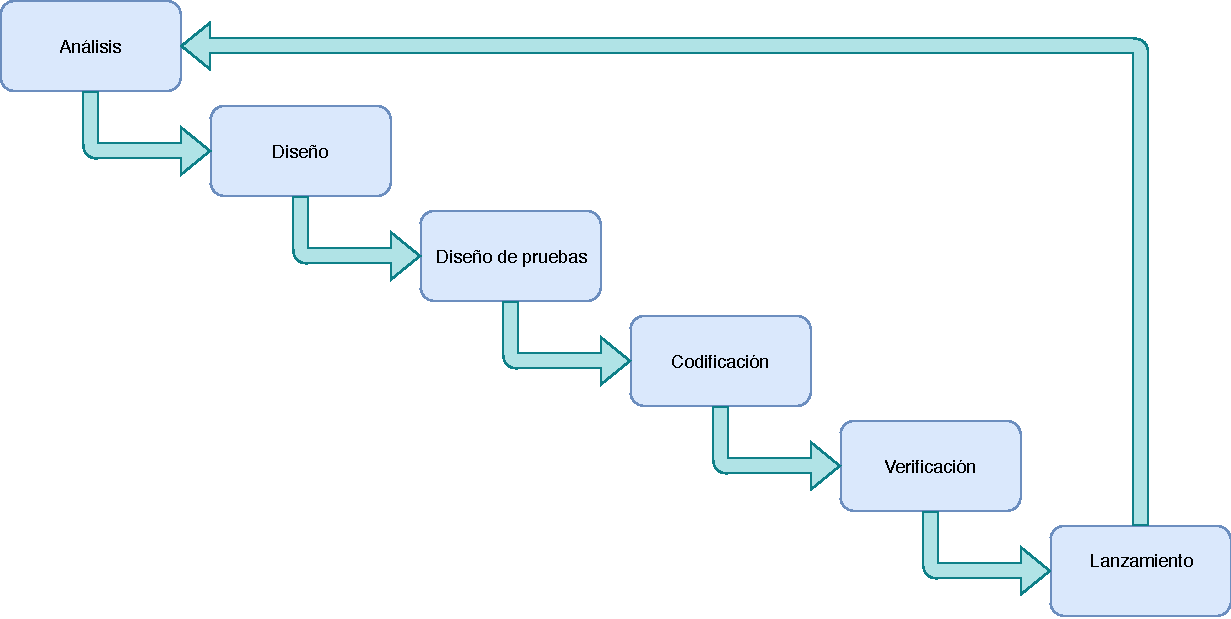
\includegraphics[width=0.7\textwidth]{Cascada.pdf}
   \caption{Ciclo cascada}
  \label{Ciclo cascada}
\end{figure}

Esta metodología es idónea para aquellos proyectos que se quieren dar fechas de entrega con mucha precisión,
 aquellos en los que se tiene claro desde el inicio que, como y cuando se va a hacer. La naturaleza de
 este TFG no permite que que se trabaje de esta manera debido a que es posible que se encuentren problemas
 durante el desarrollo del mismo y haya que buscar otras alternativas durante el mismo además de tener
 que repetir alguna de las fases con relativa frecuencia sin haber llegado a alguna de las siguientes.
 Como alternativa a este tipo de metodologías se diseño las metodologías ágiles, entre ellas
 SCRUM \cite{scrum} que será la elegida para este TFG.

\medskip
SCRUM se basa en que se pueden hacer cambios en la planificación en cualquier momento. Se planifica
 la tarea para cada sprint \footnote{Sprint: periodo de tiempo entre una y cuatro semanas en las cual
 se divide un proyecto basado en Scrum} de tal modo que en función de la duración de este los cambios
 se podrán ir adaptando en función de la necesidad del proyecto en ese momento. Además, dado que es una
 metodología ágil, favorece los cambios de última hora, esto quiere decir que permite añadir, quitar o
 modificar el trabajo planificado para ese periodo de tiempo. Para ello se tiene una cola de tareas,
 ordenadas por prioridad las cuales se van metiendo en el sprint por orden. Debido a esto encaja perfectamente
 con las características del proyecto y será la metodología escogida para llevar a cabo el mismo. Al
 ser una metodología pensada para grupos de personas y este proyecto será llevado a cabo por una única
 persona se harán modificaciones sobre este mismo para adaptarlo.

Para hacernos una idea de cual es el ciclo de vida en un proyecto de scrum podemos observar la siguiente figura:

\begin{figure}[H]
  \centering
   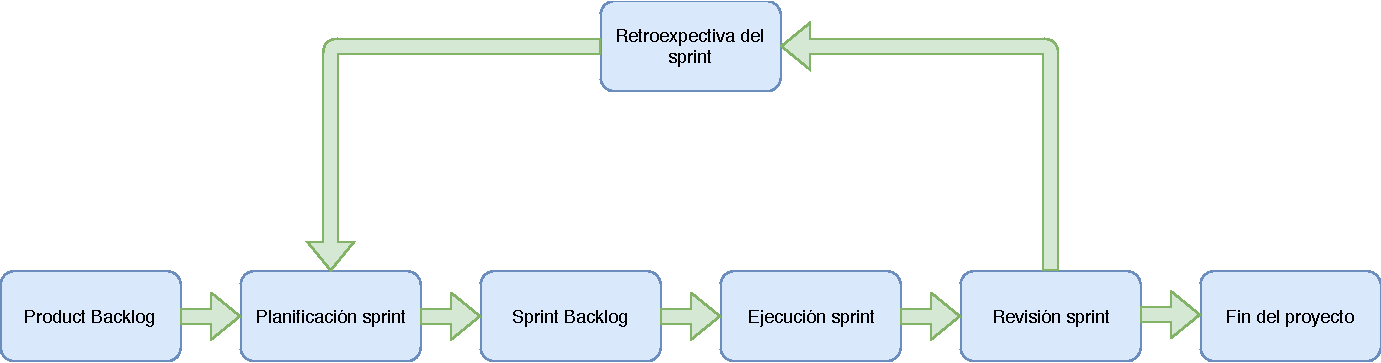
\includegraphics[width=0.7\textwidth]{Scrum.pdf}
  \caption{Ciclo SCRUM}
  \label{Ciclo SCRUM}
\end{figure}

Se eliminaron las reuniones diarias puesto que no tienen sentido en equipos de una persona,
 ya que no habrá bloqueos entre personas con sus tareas.

\bigskip

Para el product backlog se usará trello~\cite{trello} ya que nos permite crear tablones con
 notas y estas notas serán las tareas a realizar, ordenadas de arriba a abajo según su prioridad.
 Además se usará esta plataforma para saber el avance de cada tarea. Cada tarea tendrá una checklist
 compuesta por tres elementos. Estos elementos servirán para indicar el estado de la tarea. Dichos
 elementos serán \textit{tarea de sprint}, \textit{en desarrollo} y \textit{terminada}. En la \textbf{tabla 3}
 se puede ver una estimación inicial de sprints teniendo estos una duración de tres semanas.


\begin{center}
   \textbf{Tabla 3}: Planificación estimada del proyecto\\[1em]
   \rowcolors{1}{white}{sombra}
   \begin{tabular}{p{.30\textwidth} p{.20\textwidth} p{.30\textwidth}}
        \hline
		\textbf{Línea temporal} & \textbf{Duración}  & \text{Temática}\\
		\hline
		    \textbf{14/01/2019 - 01/02/2019} & Sprint 1 & Desarrollo sistema experto\\
		    \textbf{04/02/2019 - 22/02/2019} & Sprint 2 & Desarrollo sistema experto \\
		    \textbf{25/02/2019 - 15/03/2019} & Sprint 3 & Desarrollo sistema experto y desarrollo modelo aprendizaje\\
		    \textbf{18/03/2019 - 05/04/2019} & Sprint 4 & Desarrollo modelo aprendizaje\\
		    \textbf{05/04/2019 - 26/04/2019} & Sprint 5 & Desarrollo modelo aprendizaje\\
		    \textbf{29/04/2019 - 17/05/2019} & Sprint 6 & Desarrollo modelo aprendizaje y Desarrollo aplicación web\\
		    \textbf{20/05/2019 - 07/06/2019} & Sprint 7 & Desarrollo aplicación web\\
		    \textbf{10/05/2019 - 28/06/2019} & Sprint 8 & Desarrollo aplicación web\\
		\hline
   \end{tabular}
\end{center}


Respecto a la metodología elegida para el desarrollo del sistema experto será la siguiente:
\begin{itemize}
  \setlength\itemsep{1pt}
  \item Estudio de viabilidad. Este estudio será llevado a cabo mediante el test de Slagel.
  \item Adquisición de conocimiento. Se obtendrá conocimiento sobre el tema a tratar basandonose sobre todo en entrevistas a expertos de la materia.
  \item Conceptualización. Se plasmará de una forma entendible todo el conocimiento adquirido.
  \item Representación del conocimiento. Esta representación se mostrara en forma de reglas.
  \item Evaluación. Conclusiones del sistema experto.
\end{itemize}

Respecto a la metodología seguida para el desarrollo del modelo de aprendizaje será la siguiente:
\begin{itemize}
  \setlength\itemsep{1pt}
  \item Adquisición datos.
  \item Tratamiento datos.
  \item Procesamiento datos.
  \item Obtener conocimiento.
\end{itemize}

\newpage
\section{Medios que se pretende utilizar}
A continuación se detallan los medios hardware y software que se utilizan a lo largo del desarrollo del TFG

\subsection{Medios hardware}
El equipo hardware para la realización del proyecto es un PC sobremesa de las siguientes características:
 Procesador: Intel Core i5-8600K 3.6GHz; Memoria DDR4 3200 PC4-25600 8GB 2x4GB CL16; Gráficos: Gigabyte
 GeForce GTX 1060 Windforce OC 6GB GDDR5.
\subsection{Medios software}
\begin{itemize}
    \item Lenguajes de programación:
    \begin{itemize}
        \item Python~\cite{python}, lenguaje multiparadigma fuertemente tipado utilizado para la obtención y procesamiento de datos.
        \item CLIPS \cite{clips}, lenguaje de programación multiparadigma utilizado para la representación plasmar la representación del conocimiento.
        \item LaTeX \cite{latex}, sistema de composición de textos utilizado para generar la documentación.
        \item Ruby on Rails \cite{ror}, framework de Ruby que sigue el paradigma MVC \footnote{Modelo Vista Controlador} utilizado para el desarrollo de la aplicación web.
    \end{itemize}
    \item Librerías:
    \begin{itemize}
        \item Python NumPy \cite{numpy}. Librería usada para el tratamiento de datos
        \item Python Matplotlib \cite{matplotlib}. Librería utilizada para mostrar gráficos 2D
        \item BeatifulSoup4 \cite{beatifulsoup}. Librería cuyo uso está destinado a la obtención de datos mediante web scrapping.
    \end{itemize}
    \item Entorno de desarrollo:
    \begin{itemize}
        \item Anaconda \cite{anaconda}, Software de gestión de paquetes de python y R
        \item Spyder \cite{spyder}, IDE para el desarrollo de aplicaciónes en python
        \item Google Chrome \cite{chrome}, navegador utilizado para consultas
        \item Firefox \cite{firefox}, navegador utilizado para obtención de datos
        \item Overleaf \cite{overleaf}, aplicación web utilizada para generar la documentación
    \end{itemize}
    \item Herramientas de gestión y desarrollo:
    \begin{itemize}
        \item Trello, aplicación web utilizada para la gestión de tareas
        \item Github \cite{github}, aplicación web utilizada para el control de versiones \cite{git}
        \item Toggl \cite{toggl}, aplicación web utilizada para la gestión y control del tiempo empleado en cada tarea.
        \item Draw.io \cite{drawio}, aplicación web utilizada para la creación de imágenes y diagramas.
    \end{itemize}
\end{itemize}

\newpage
\addcontentsline{toc}{section}{Bibliografía} % Para añadir la bibliografía al TOC 

\nocite{*} % Se incluyen todas las fuentes bibliográficas aunque no hayan sido citadas en el texto. En este caso la bibliografía es en realidad una lista de fuentes de consulta y así se podría indicar.
\printbibliography[title=Bibliografía]

\end{document}
